\documentclass[tikz,border=2pt]{standalone}
\usetikzlibrary{calc}
\usetikzlibrary{intersections}
\usetikzlibrary{patterns}
\usepackage{bm}

\begin{document}

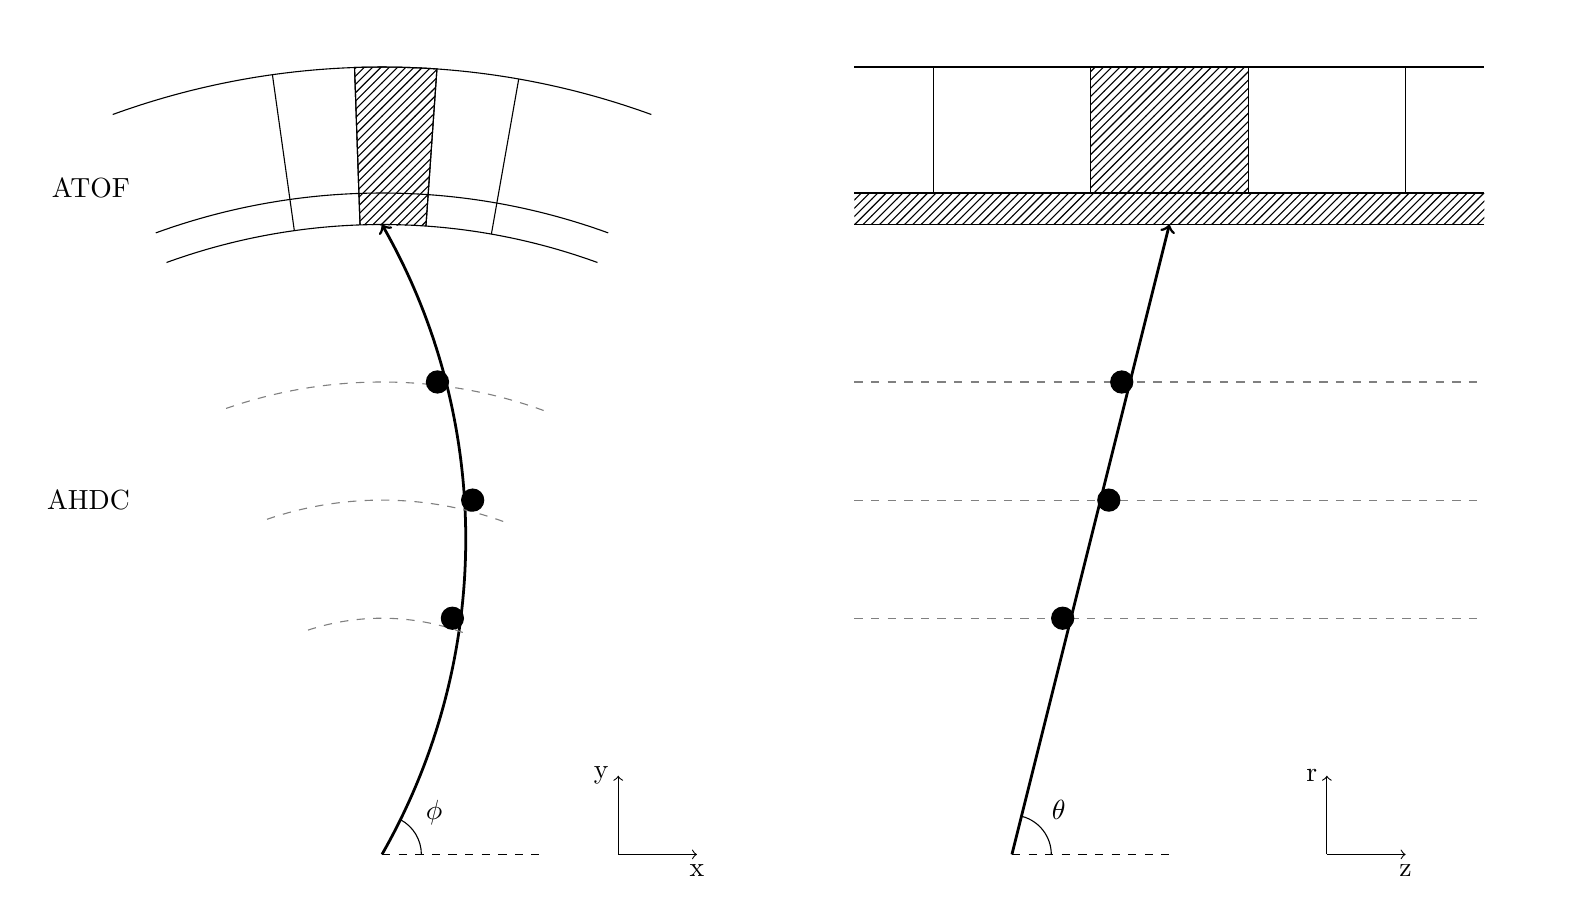
\begin{tikzpicture}%[scale=4, very thin]

    % clip the drawing
    \clip (-4.5,-0.5) rectangle (15,10.5);
    
    %% XY view
    \begin{scope}
        %%%%%%%%%%%%%%%%%%%%%%%%%%
        % Draw track
        %%%%%%%%%%%%%%%%%%%%%%%%%%
        % --- points A, B, C
        \def\xA{0}
        \def\yA{0}
        \def\xB{1}
        \def\yB{5}
        \def\xC{0}
        \def\yC{8}
        % --- Calcul du déterminant ---
        \pgfmathsetmacro{\D}{2*(\xA*(\yB-\yC) + \xB*(\yC-\yA) + \xC*(\yA-\yB))}
        % --- Centre du cercle ---
        \pgfmathsetmacro{\xc}{
        ((\xA*\xA+\yA*\yA)*(\yB-\yC) +
        (\xB*\xB+\yB*\yB)*(\yC-\yA) +
        (\xC*\xC+\yC*\yC)*(\yA-\yB))/\D
        }
        \pgfmathsetmacro{\yc}{
        ((\xA*\xA+\yA*\yA)*(\xC-\xB) +
        (\xB*\xB+\yB*\yB)*(\xA-\xC) +
        (\xC*\xC+\yC*\yC)*(\xB-\xA))/\D
        }
        % --- Rayon ---
        \pgfmathsetmacro{\r}{sqrt((\xA-\xc)^2 + (\yA-\yc)^2)}
        % --- Angles pour l'arc ---
        \pgfmathsetmacro{\angleA}{atan2(\yA-\yc,\xA-\xc)}
        \pgfmathsetmacro{\angleC}{atan2(\yC-\yc,\xC-\xc)}
        % arc entre A et C
        \draw[line width=1pt,black,->,name path=track] (\xc,\yc) ++(\angleA:\r) arc (\angleA:\angleC:\r);
        \coordinate (atof) at ($(\xc,\yc)+(\angleC:\r)$);        
        
        %%%%%%%%%%%%%%%%%%%%%%%%%%
        % AHDC hits
        %%%%%%%%%%%%%%%%%%%%%%%%%%
        \path[name path=layer1] (0,1.5) -- (5,1.5);
        \path[name path=layer2] (0,3) -- (5,3);
        \path[name path=layer3] (0,4.5) -- (5,4.5);
        \path[name path=layer4] (0,6) -- (5,6);

        %\draw [gray, dashed] (70:1.5) arc (70:110:1.5);
        \draw [gray, dashed] (70:3) arc (70:110:3);
        \draw [gray, dashed] (70:4.5) arc (70:110:4.5);
        \draw [gray, dashed] (70:6) arc (70:110:6);
        
        \path[name intersections={of=track and layer1, by=P1}];
        \path[name intersections={of=track and layer2, by=P2}];
        \path[name intersections={of=track and layer3, by=P3}];
        \path[name intersections={of=track and layer4, by=P4}];

        %\filldraw [fill=black] ($(P1)+(3pt,0)$) circle [radius=4pt];
        \filldraw [fill=black] ($(P2)-(3pt,0)$) circle [radius=4pt];
        \filldraw [fill=black] ($(P3)+(3pt,0)$) circle [radius=4pt];
        \filldraw [fill=black] ($(P4)-(3pt,0)$) circle [radius=4pt];

        %%%%%%%%%%%%%%%%%%%%%%
        % Draw ATOF
        %%%%%%%%%%%%%%%%%%%%%%
        \draw (0,0) ++(70:8) arc (70:110:8); % S1
        \draw (0,0) ++(70:8.4) arc (70:110:8.4); % S2
        \draw (0,0) ++(70:10) arc (70:110:10); % S3
        \node [left] at (110:9) {ATOF};
        \node [left] at (110:9 |- 0,4.5) {AHDC};
        %\node  at (110:9 |- 0,4.25) {\tiny only 3 layers represented};

        \draw (80:8) -- (80:10);
        \draw (86:8) -- (86:10);
        \draw (92:8) -- (92:10);
        \draw (98:8) -- (98:10);
        \filldraw [pattern color=black, draw=black, pattern=north east lines] (86:8) -- (86:10) arc (86:92:10) -- (92:8);
        %\draw (80:8) -- (80:10);

        % draw axis
        \draw [->] (3,0) -- (4,0) node [below] {x};
        \draw [->] (3,0) -- (3,1) node [left] {y};

        % draw phi
        \draw [dashed] (0,0) -- (2,0);
        \draw (0,0) ++(0:0.5) arc (0:62:0.5);
        \node [above right] at (30:0.5) {$\phi$};
    \end{scope}

    %% ZR view
    \begin{scope}[xshift=8cm]
        % draw track
        \draw[line width=1pt,black,->,name path=track] (0,0) -- (2,8);
        % draw atof
        \draw (-2,8) -- (6,8); %S1
        \draw (-2,8.4) -- (6,8.4); %S2
        \draw (-2,10) -- (6,10); %S3

        \draw (-1,8.4) -- (-1,10);
        \draw (1,8.4) -- (1,10);
        \draw (3,8.4) -- (3,10);
        \draw (5,8.4) -- (5,10);

        \filldraw [pattern color=black, draw=black, pattern=north east lines] (1,8.4) -- (1,10) -- (3,10) -- (3,8.4) -- cycle;
        \fill [pattern color=black, pattern=north east lines] (-2,8) -- (-2,8.4) -- (6,8.4) -- (6,8) -- cycle;

        % draw AHDC
        %\draw [gray, dashed, name path=layer1] (-2,1.5) -- (6,1.5);
        \draw [gray, dashed, name path=layer2] (-2,3) -- (6,3);
        \draw [gray, dashed, name path=layer3] (-2,4.5) -- (6,4.5);
        \draw [gray, dashed, name path=layer4] (-2,6) -- (6,6);

        %\path[name intersections={of=track and layer1, by=P1}];
        \path[name intersections={of=track and layer2, by=P2}];
        \path[name intersections={of=track and layer3, by=P3}];
        \path[name intersections={of=track and layer4, by=P4}];

        %\filldraw [fill=black] ($(P1)+(3pt,0)$) circle [radius=4pt];
        \filldraw [fill=black] ($(P2)-(3pt,0)$) circle [radius=4pt];
        \filldraw [fill=black] ($(P3)+(3pt,0)$) circle [radius=4pt];
        \filldraw [fill=black] ($(P4)-(3pt,0)$) circle [radius=4pt];

         % draw axis
        \draw [->] (4,0) -- (5,0) node [below] {z};
        \draw [->] (4,0) -- (4,1) node [left] {r};

        % draw theta
        \draw [dashed] (0,0) -- (2,0);
        \draw (0,0) ++(0:0.5) arc (0:75:0.5);
        \node [above right] at (40:0.5) {$\theta$};

    \end{scope}
\end{tikzpicture}


\end{document}